\documentclass[12pt]{report}
\usepackage{graphicx}
\usepackage{epsfig}
\begin{document}

\begin{center}
{\LARGE\bf Target Operation Manual}
\end{center}

\section{Contacts}

\noindent
Hall-B beam line expert: 

\noindent
Stepan Stepanyan: 269-7196 (office) 584-7196 (pager)

\section{\bf Target}

Figure 1 shows the HPS target. The 4$\mu$m-thick tungsten is used for 1.1 GeV and 2.2 GeV data taking, and the 8$\mu$m-thick tungsten is for 4.4 GeV and 6.6 GeV. The graphite and CH$_2$ targets are for cross section calibration.

\begin{figure}[ht!]
\centering
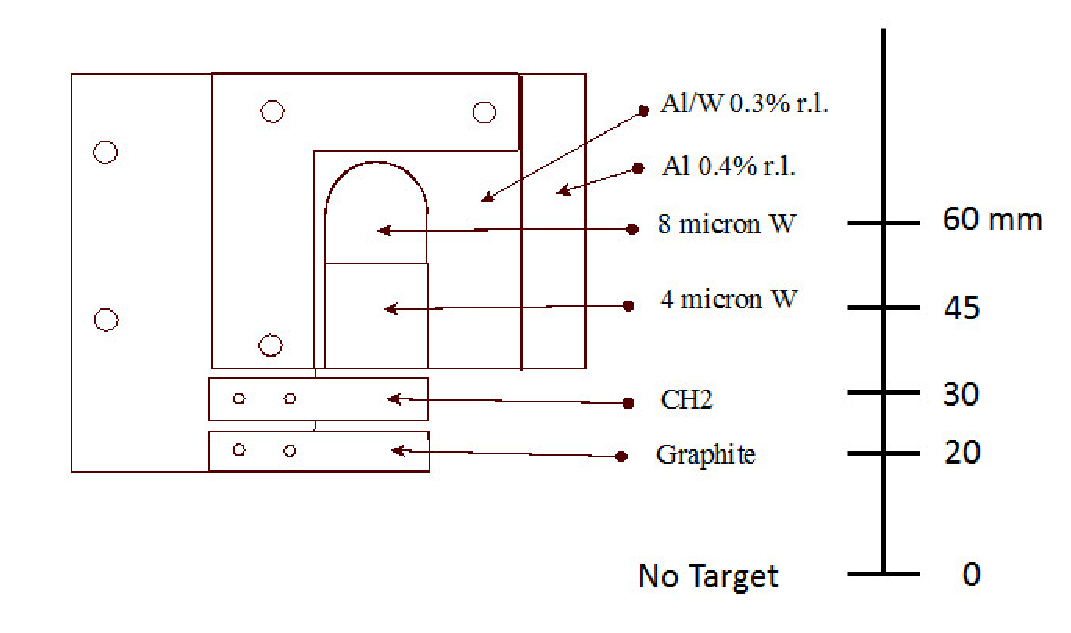
\includegraphics[width=10cm]{target.eps}
\caption{Target}
\label{target}
\end{figure}

\section{\bf Setting the target}

Target can be set by running the target GUI (Figure 2).

\begin{itemize}
\item
Type in who you are.
\item
Call MCC to turn off the beam and click ``Have you called MCC to turn off the beam?''.
\item
Hit appropriate target button.
\item 
Hit ``Remove Target'' button to remove the target.
\end{itemize}

Your name and Date and Time will be logged. The target will be placed at the nominal beam position. By providing an offset value, the target position can be adjusted vertically.

\begin{figure}[ht!]
\centering
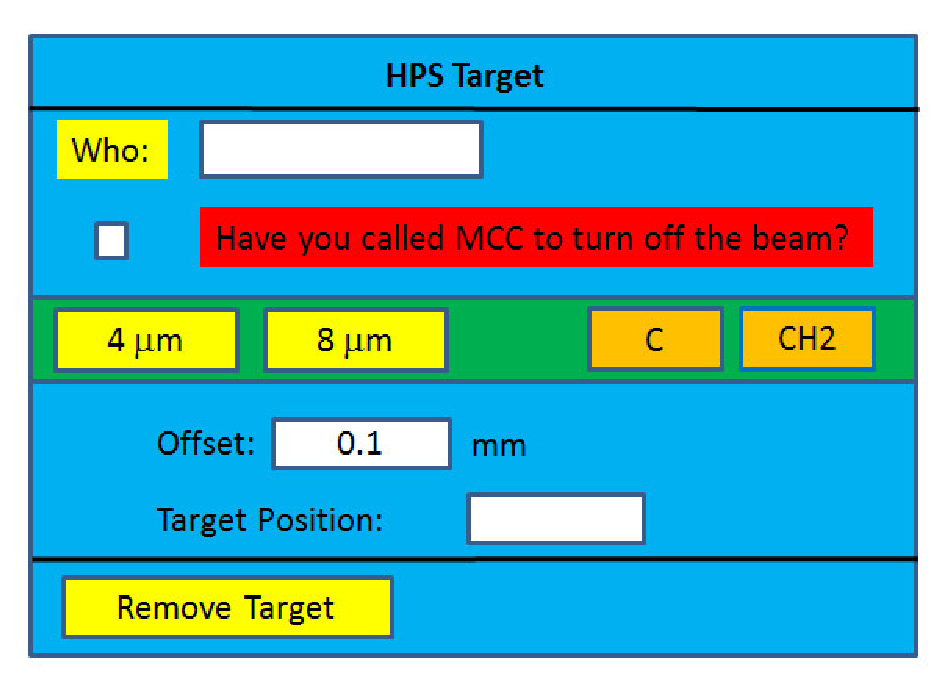
\includegraphics[width=10cm]{targetgui.eps}
\caption{Target GUI}
\label{targetgui}
\end{figure}
 

\end{document}
